\documentclass[tikz,border=5pt]{standalone}
\usepackage[UTF8]{ctex}
\usepackage{amsmath,amssymb}
\usetikzlibrary{arrows.meta,calc,angles,quotes,decorations.pathmorphing}
\definecolor{ink}{HTML}{243447}\definecolor{blue}{HTML}{2765A2}
\definecolor{green}{HTML}{3F7D5B}\definecolor{red}{HTML}{B74739}
\tikzset{body/.style={draw=ink,thick},vec/.style={draw=blue,thick,-{Latex}},guide/.style={gray!65,dashed},dim/.style={ink,{Latex}-{Latex}},line cap=round,line join=round}
\begin{document}
\begin{tikzpicture}
\fill[blue!6](0,0)circle(2.2);\draw[body](0,0)circle(2.2);
\draw[guide](-2.2,0)arc[start angle=180,end angle=0,x radius=2.2,y radius=.65];
\draw[body](2.2,0)arc[start angle=0,end angle=-180,x radius=2.2,y radius=.65];
\draw[body,fill=gray!25](0,0)circle(.4);
\draw[dim](0,0)--(-1.556,-1.556)node[midway,below left]{$R$};
\draw[ink,-{Latex}](1,-.65)--(.35,-.2)node[pos=0,above]{$r$};
\node at(0,1.35){电阻率 $\rho$};
\node[above]at(0,2.4){外球壳};
\end{tikzpicture}
\begin{tikzpicture}
\draw[body](0,0)circle(2.1)(0,0)circle(.6);
\fill[blue!15,even odd rule](0,0)circle(1.5)(0,0)circle(1.25);
\draw[blue](0,0)circle(1.25)(0,0)circle(1.5);
\draw[vec](.7,0)--(1.1,0)node[midway,above]{$I$};
\draw[vec](1.6,0)--(2.05,0);
\draw[dim](0,-.25)--(1.25,-.25)node[midway,below]{$x$};
\draw[ink](1.36,-.6)--(1.7,-1.2)node[right]{$\mathrm dx$};
\node at(-1.2,2.35){面积 $4\pi x^2$};
\node at(0,-2.5){$\mathrm d\mathcal R=\rho\,\mathrm dx/(4\pi x^2)$};
\end{tikzpicture}
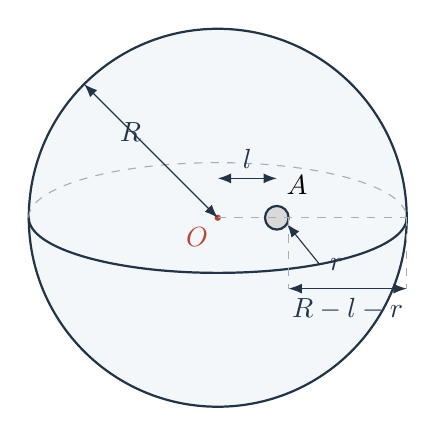
\begin{tikzpicture}
\fill[blue!5](0,0)circle(2.4);\draw[body](0,0)circle(2.4);
\draw[guide](-2.4,0)arc[start angle=180,end angle=0,x radius=2.4,y radius=.7];
\draw[body](2.4,0)arc[start angle=0,end angle=-180,x radius=2.4,y radius=.7];
\fill[red](0,0)circle(.04)node[below left]{$O$};
\draw[body,fill=gray!30](.75,0)circle(.15);
\node[above right]at(.75,.17){$A$};
\draw[guide](0,0)--(2.4,0);
\draw[dim](0,.5)--(.75,.5)node[midway,above]{$l$};
\draw[ink,-{Latex}](1.3,-.6)--(.88,-.08)node[pos=0,right]{$r$};
\draw[dim](0,0)--(-1.697,1.697)node[midway,above left]{$R$};
\draw[dim](.9,-.9)--(2.4,-.9)node[midway,below]{$R-l-r$};
\draw[guide](.9,0)--(.9,-.9)(2.4,0)--(2.4,-.9);
\end{tikzpicture}
\begin{tikzpicture}
\draw[body](0,0)circle(2);
\draw[guide](-2.3,0)--(5,0);
\fill[red](0,0)circle(.04)node[below left]{$O$};
\fill[blue](.9,0)circle(.045)node[above]{$A,\ I$};
\fill[green](4.444,0)circle(.045)node[above]{$A',\ I'=-RI/l$};
\coordinate(P)at(1,1.732);
\fill[ink](P)circle(.04)node[above]{$P$};
\draw[blue](.9,0)--(P)node[midway,left]{$|P-A|$};
\draw[green](4.444,0)--(P)node[midway,above]{$|P-A'|$};
\draw[dim](0,-2.5)--(4.444,-2.5)node[midway,below]{$d=R^2/l$};
\draw[dim](0,-.5)--(.9,-.5)node[midway,below]{$l$};
\node[below]at(-1,-1.8){$V=0$};
\node at(1,-3.5){过两球心的截面；镜像点位于实际导体之外};
\end{tikzpicture}
\end{document}
